% !TEX root = CFAST_Users_Guide.tex

\chapter{Simulation Environment}

The \textbf{Simulation} tab defines initial conditions, numerical parameters, and other global miscellaneous parameters.

\begin{figure}[ht]
\centering

\includegraphics[width=6.5in]{SCRIPT_FIGURES/Environment_Tab}
\caption[The Simulation Tab]{The Simulation Tab.}
\end{figure}

\section{Title}
\label{info:HEAD}

\begin{description}
\item[Title] (namelist: \ct{TITLE}) Optional title that may consist of letters, numbers, and/or symbols and may be up to 50 characters. All output files will be tagged with this character string. Note that the \textbf{Title} is not used to name the text input file.
\end{description}
The \ct{HEAD} line of the input file will contain the \textbf{Title} and a \ct{VERSION} number that is used to detect older versions of the software.



\section{Simulation Times}
\label{info:TIME}

\begin{description}
\item[Simulation Time] (default: 900 s; namelist: \ct{SIMULATION}): Duration of the simulation. The maximum value for this input is 86400~s (1~day).

\item[Text Output Interval] (default: 60 s; namelist: \ct{PRINT}): Time interval between diagnostic outputs. If equal to zero, no output values will appear.

\item[Spreadsheet Output Interval] (default: 15 s; namelist: \ct{SPREADSHEET}): Time interval between outputs to comma-delimited spreadsheet files. A value greater than zero must be used if the spreadsheet files are desired.

\item[Smokeview Output Interval] (default: 15 s; namelist: \ct{SMOKEVIEW}): Time interval between outputs to the visualization program Smokeview.  A value greater than zero must be used if the Smokeview output is desired.
\end{description}


\section{Simulation Conditions}
\label{info:INIT}

Ambient conditions define the starting environment. The initial pressure profile is calculated using a lapse rate based on the NOAA/NASA tables~\cite{GPO:Atmosphere}. The specified ambient pressure is taken at relative height of zero. The temperature and pressure must then be measured at that position.  Another possible choice would be the pressure and temperature at sea level, with the structure elevations then given with respect to mean sea level.  This is also acceptable, but somewhat more tedious in specifying the construction of a structure.  Either of these choices works though, so long as they are consistent. Usually, the station elevation is set to zero and the pressure to ambient. The effect of changing these values is minor. Note that the equations implemented in the model are not designed to handle negative elevations and altitudes.
\begin{description}
\item[Interior Temperature] (default: 20~\unit{\degreeCelsius}; namelist: \ct{INTERIOR_TEMPERATURE}): Initial temperature inside the structure at the station elevation.

\item[Humidity] (default: 50 \%; namelist: \ct{RELATIVE_HUMIDITY}): The initial relative humidity, only specified for the interior.  This is converted to kilograms of water per cubic meter as an initial condition for both the interior and exterior of the structure.

\item[Exterior Temperature] (default: 20~\unit{\degreeCelsius}; namelist: \ct{EXTERIOR_TEMPERATURE}): Initial temperature outside the structure at the station elevation.

\item[Pressure] (default: 101325 Pa; namelist: \ct{PRESSURE}): Initial pressure inside and outside the structure at the station elevation.

\item[O$_2$ mass fraction] (default: 0.23~\unit{kg/kg}; namelist: \ct{INTERIOR_O2_MASS_FRACTION} and \ct{EXTERIOR_O2_MASS_FRACTION}):
Initial values for ambient oxygen mass fraction inside and outside the structure. The default nitrogen mass fraction is one minus the default oxygen mass fraction.
\end{description}



\section{Miscellaneous}
\label{info:MISC}

Keywords associated with global parameters are organized in the miscellaneous namelist group.
\begin{description}
\item[Adiabatic Compartment Surfaces] (default: False; namelist: \ct{ADIABATIC}) When this box is checked, all of the compartment surfaces are assumed to be perfect insulators and material properties are ignored. This feature is useful when designing an experiment in which it is assumed that there is no heat transfer to the walls of the compartments.

\item[Lower Oxygen Limit] (default: 15~\%; namelist: \ct{LOWER_OXYGEN_LIMIT}):  Oxygen volume fraction below which combustion is suppressed following a smooth transitional curve.

\item[Maximum Solver Iterations] (default: $-1$ (unlimited); namelist: \ct{MAX_ITERATION}) Maximum number of iterations for the equation solver.

\item[Maximum Time Step] (default: 1 s; namelist: \ct{MAX_TIME_STEP}): CFAST automatically adjusts the time step for the solution of the differential equations to satisfy pre-defined error tolerances. This parameter caps the time step and is normally left at the default value. For cases where the solver fails to converge to a solution, the value can be reduced which might allow the simulation to successfully complete.

\item[Overwrite] (default: True; namelist: \ct{OVERWRITE}) Controls whether existing output files may be overwritten.

\item[Extinction Coefficient] (default: 8700 (flaming), 4400 \unit{m^2/kg} (smoldering); namelist: \ct{SPECIFIC_EXTINCTION(2)}) Specific-extinction coefficients for flaming and smoldering combustion, respectively.
\end{description}





\chapter{Thermal Properties}
\label{info:MATL}

The thermophysical properties of materials used for compartment surfaces or targets are set in the Thermal Properties tab.

\begin{figure}[ht]
\centering

\includegraphics[width=6.5in]{SCRIPT_FIGURES/Thermal_Properties_Tab}
\caption[The CFAST Thermal Properties Tab]{The CFAST Thermal Properties Tab.}
\end{figure}

\section{Adding Thermal Properties}


CFAST does not include predefined thermal properties for compartment materials. Thus, the user needs to define materials for use within a specific simulation. These may be taken from other simulations or entered directly from reference sources or test results. Clicking the \textbf{Add} button and assigning values to the following list of properties will create a set of thermal properties associated with a material used in a compartment or a target. The thermophysical properties are specified at one condition of temperature, humidity, etc.
\begin{description}
\item[Material] (namelist: \ct{MATERIAL}) A descriptive name for the material.

\item[ID] (namelist: \ct{ID}) A one-word (no more than 8 characters) {\it unique} identifier for the material.  This identifier should not contain any spaces and is used in other CFAST inputs to identify the particular material referenced.

\item[Conductivity] (default units: \unit{kW/(m.K)}; namelist: \ct{CONDUCTIVITY}) Thermal conductivity for the material. Note the units---this property is often listed in units of W/(m$\cdot$K).

\item[Specific Heat] (default units: \unit{kJ/(kg.K)}; namelist: \ct{SPECIFIC_HEAT}) Specific heat for the material.

\item[Density] (default units: \unit{kg/m^3}; namelist: \ct{DENSITY}) Density of the material.

\item[Thickness] (default units: m; namelist: \ct{THICKNESS}) Thickness of the material. A compartment surface may override this value; targets use the material value unless an alternative value is given.

\item[Emissivity] (default: 0.9; namelist: \ct{EMISSIVITY}) Emissivity of the material surface; that is, the fraction of the radiative flux that is absorbed by the material.

\item[FYI] (namelist: \ct{FYI}) Optional note, for example, a reference.
\end{description}



\section{Adding Thermal Properties From Another File}

The \textbf{From File} button imports thermal properties from one or more existing CFAST input files. Select the desired files with extensions \ct{.in} or \ct{.cfast}. CEdit reads the \ct{MATL} records from all selected files and displays the available materials in a single list. Use the checkboxes or the \textbf{Select All} and \textbf{Deselect All} buttons to choose the materials to add, then click \textbf{OK}. Materials whose \ct{ID}s already exist in the current case are skipped. CEdit reports the numbers of materials added and duplicate \ct{ID}s are skipped.





\chapter{Compartments}

The \textbf{Compartments} tab defines the geometry and lining materials of the compartments, which at a minimum require a width, depth, and height. The maximum number of compartments is 100. The usual assumption is that compartments are rectangular parallelepipeds, but other shapes can be modeled via equivalent floor area and perimeter.

\begin{figure}[h!]
\begin{center}

\includegraphics[width=6.5in]{SCRIPT_FIGURES/Compartment_Geometry_Tab}
\caption[The CFAST Compartments Tab]{The CFAST Compartments Tab.}
\end{center}
\end{figure}

In CEdit the default room has a width of 3.6~m, a depth of 2.4~m, a height of 2.4~m, and an absolute position of (0,0,0). The ceiling, walls, and floor are set to \ct{OFF} by default, meaning no materials are assigned. The normal two-zone model is selected; the shaft (single-zone) and corridor options are off by default.

\begin{figure}[ht]
\begin{tabular*}{\textwidth}{@{}c@{\extracolsep{\fill}}c@{}}
\resizebox{3.35in}{!}{% !TEX root = ../CFAST_Users_Guide.tex
%
% Requires:
%   %
% CFAST compartment coordinate system.
% The face lettering is transformed with the plane itself, rather
% than merely rotated in the page.

\begin{tikzpicture}[
  x={(0.78cm,0cm)},
  y={(0.35cm,0.23cm)},
  z={(0cm,0.78cm)},
  >=Stealth, line cap=round, line join=round,
  every node/.style={font=\small}
]
  \def\W{4}
  \def\D{4}
  \def\H{4}

  % ------------------------------------------------------------
  % BOX
  %
  % From this viewpoint the y=0 (Front) and x=W (Right) faces
  % are visible.  The x=0 (Left) and y=D (Rear) faces are hidden.
  % Consequently, their complete perimeter edges are dashed.
  % ------------------------------------------------------------

  % Hidden edges: the bottom-left-to-rear edge, the rear-left
  % vertical edge, and the entire rear bottom edge are hidden.
  \draw[dashed, line width=1pt]
    (0,0,0)--(0,\D,0)
    (0,\D,0)--(0,\D,\H)
    (0,\D,0)--(\W,\D,0);

  % Visible edges: all top edges are visible from this viewpoint.
  \draw[line width=1pt]
    % Front face
    (0,0,0)--(\W,0,0)
    (\W,0,0)--(\W,0,\H)
    (\W,0,\H)--(0,0,\H)
    (0,0,\H)--(0,0,0)
    % Right face
    (\W,0,0)--(\W,\D,0)
    (\W,\D,0)--(\W,\D,\H)
    (\W,\D,\H)--(\W,0,\H)
    % visible top/rear edges
    (0,0,\H)--(0,\D,\H)
    (0,\D,\H)--(\W,\D,\H);

  % ------------------------------------------------------------
  % COORDINATE AXES
  % ------------------------------------------------------------

  \draw[line width=1.4pt,->]
    (0,0,0)--(5.4,0,0)
    node[below right] {$X$};

  \draw[line width=1.4pt,->]
    (0,0,0)--(0,6.0,0)
    node[right] {$Y$};

  \draw[line width=1.4pt,->]
    (0,0,0)--(0,0,4.8)
    node[above right] {$Z$};

  \node[below left] at (0,0,0) {$(0,0,0)$};

  % ------------------------------------------------------------
  % DIMENSIONS
  % ------------------------------------------------------------

  \node[below] at (2,0,0) {Width};
  \node[rotate=90] at (-0.42,0,2) {Height};
    \begin{scope}[canvas is yz plane at x=4.7]
    \node[transform shape] at (2,0.15) {Depth};
  \end{scope}

  % ------------------------------------------------------------
  % FACE LABELS
  %
  % "transform shape" is essential: it causes the glyphs themselves
  % to undergo the affine transformation of the plane.  Thus the
  % labels look like they are printed on the corresponding faces.
  %
  % Front/Rear are X-Z planes.
  % Left/Right are Y-Z planes.
  % ------------------------------------------------------------

  % Front: visible face y=0
  \begin{scope}[canvas is xz plane at y=0]
    \node[red, font=\Large, transform shape] at (1.35,1.75) {Front};
  \end{scope}

  % Rear: hidden face y=D
  \begin{scope}[canvas is xz plane at y=\D]
    \node[red, font=\Large, transform shape] at (1.35,2.35) {Rear};
  \end{scope}

  % Left: hidden face x=0
  \begin{scope}[canvas is yz plane at x=0]
    \node[red, font=\Large, transform shape] at (2,2) {Left};
  \end{scope}

  % Right: visible face x=W
  \begin{scope}[canvas is yz plane at x=\W]
    \node[red, font=\Large, transform shape] at (2,2) {Right};
  \end{scope}

\end{tikzpicture}
} &
\resizebox{3.10in}{!}{% !TEX root = ../CFAST_Users_Guide.tex

% Oblique projection used by the original CFAST compartment diagrams.
% The lower and upper boxes are constructed from actual model dimensions and offsets.
\begin{tikzpicture}[
  x={(0.72cm,0cm)}, y={(0.34cm,0.22cm)}, z={(0cm,0.72cm)},
  >=Stealth, line cap=round, line join=round,
  every node/.style={font=\small}
]
  % Lower compartment: 4 m wide, 4 m deep, and 2.3 m high.
  \draw[line width=1pt]
    (0,0,0)--(4,0,0)--(4,4,0)--(0,4,0)--cycle
    (0,0,2.3)--(4,0,2.3)--(4,4,2.3)--(0,4,2.3)--cycle
    (0,0,0)--(0,0,2.3)
    (4,0,0)--(4,0,2.3)
    (4,4,0)--(4,4,2.3)
    (0,4,0)--(0,4,2.3);

  % Upper compartment: 2 m wide, 5 m deep, and 2.3 m high.
  % Its front-left-bottom corner is offset 2 m in Y and 2.3 m in Z.
  \draw[line width=1pt]
    (0,2,2.3)--(2,2,2.3)--(2,7,2.3)--(0,7,2.3)--cycle
    (0,2,4.6)--(2,2,4.6)--(2,7,4.6)--(0,7,4.6)--cycle
    (0,2,2.3)--(0,2,4.6)
    (2,2,2.3)--(2,2,4.6)
    (2,7,2.3)--(2,7,4.6)
    (0,7,2.3)--(0,7,4.6);

  \draw[line width=1.4pt,->] (0,0,0)--(6.1,0,0) node[below right] {$X$};
  \draw[line width=1.4pt,->] (0,0,0)--(0,5.8,0) node[right] {$Y$};
  \draw[line width=1.4pt,->] (0,0,0)--(0,0,5.4) node[above right] {$Z$};
  \node[below left] at (0,0,0) {$(0,0,0)$};

  \node at (2,0,0.30) {4 m};
  \node[rotate=90] at (0.35,0,1.15) {2.3 m};
  \node[rotate=33] at (4.5,2.15,0.0) {4 m};
  \node[rotate=33] at (0,4.50,4.90) {5 m};
  \node[rotate=90] at (0.35,2,3.45) {2.3 m};
  \node[rotate=33] at (0,1.0,2.7) {2 m};
  \node[font=\footnotesize] at (1.5,2,2.58) {2 m};
\end{tikzpicture}
} \\
Compartment Size & Compartment Position
\end{tabular*}
\caption[Compartment Orientation and Positioning in CFAST]{Compartment Orientation and Positioning in CFAST.}
\label{fig:compartment_positioning}
\end{figure}



\section{Geometry}
\label{info:COMP}
\label{Compartment_Geometry}

Compartments in CFAST are most typically defined by a width, depth, and height.  If desired, compartments can be prescribed by the cross-sectional area of the compartment as a function of height from floor to ceiling for other shapes. The absolute position of the compartment with respect to a single structure reference point can be defined to ease visualization or to allow exact placement of vents and surfaces relative to other compartments in a detailed calculation. This specification is important for positioning the compartments for visualization in Smokeview.
\begin{description}
\item[ ID:] (namelist: \ct{ID}) Compartments are identified by a unique name, for which spaces are allowed.

\item[Width] (default: 3.6 m; namelist: \ct{WIDTH}) Compartment width as measured on the $x$ axis from the origin of the compartment.

\item[Depth] (default: 2.4 m; namelist: \ct{DEPTH}) Compartment depth as measured on the $y$ axis from the origin of the compartment.

\item[Height] (default: 2.4 m; namelist: \ct{HEIGHT})  Compartment height as measured on the $z$ axis from the origin of the compartment.

\item[X Position, Y Position, Z Position] (default: (0,0,0) m; namelist: \ct{ORIGIN(1:3)}) Coordinates of the lower, left, front corner of the compartment. All coordinates for all compartments must be greater than or equal to zero to facilitate visualization by Smokeview.
\end{description}



\section{Materials}
\label{info:COMP2}

To calculate heat loss through the ceiling, walls, and floor of a compartment, material properties must be specified. Separate properties can be specified for the ceiling and floor, but the four walls all must have the same set of properties. The thermophysical properties are described in Sec.~\ref{info:MATL}. If the thermophysical properties of the surfaces are not specified, they will be treated as adiabatic, i.e. no heat transfer. The back surfaces of compartments are assumed to be exposed to ambient conditions.

\begin{description}
\item[Surface Construction: Ceiling, Walls, Floor] (namelist: \ct{CEILING_MATL_ID}, \ct{WALL_MATL_ID}, \ct{FLOOR_MATL_ID}) As many as three layers of materials can make up the compartment linings, with the surface layer specified first.

\item[Ceiling, Walls, Floor Thickness] (default: Materials tab \textbf{Thickness}; namelist: \ct{CEILING_THICKNESS}, \ct{WALL_THICKNESS}, \ct{FLOOR_THICKNESS}): Thickness of each of the layers of the compartment surfaces.
\end{description}





\section{Modeling a Compartment as a Tall Shaft or Long Corridor}
\label{info:COMP3}

\begin{description}
\item[Normal (Two-zone model)] Conditions in the compartment are calculated with the normal two-zone approach. This is the default model used for a compartment.

\item[Shaft (Single-zone model)] (namelist: \ct{SHAFT=T}) Conditions in the compartment are calculated as a single well-mixed zone. A single zone approximation may be appropriate for compartments away from the fire, where the two-zone layer stratification is less pronounced than in compartments near the fire, or in situations where the stratification does not occur, such as elevators, shafts, or stairwells.

\item[Corridor (Revised ceiling jet)] (namelist: \ct{HALL=T}) Conditions in the compartment are calculated with the normal two-zone approach, but ceiling jet temperatures are calculated with an empirical model that constrains the upper layer to a narrow passage. This feature will impact, for example, detectors, sprinklers, and targets near the ceiling in corridors.
\end{description}




\section{Defining Variable Compartment Area}
\label{info:COMP4}

The \textbf{Compartments} tab includes a table entitled \textbf{Variable Cross-sectional Area} for defining a compartment whose horizontal cross-sectional area is a function of height:
\begin{description}
\item[Height] (namelist: \ct{CROSS_SECT_HEIGHTS(:)}) Height (m) off the floor of the compartment.
\item[Area] (namelist: \ct{CROSS_SECT_AREAS(:)}) Cross-sectional area (\unit{m^2}) at the corresponding height.
\end{description}
Cross-sectional area values should be input in order by ascending height. If the first height value is not zero (i.e., at floor level), the cross-sectional area is assumed constant from the floor to the height specified in the first cross-sectional area value. Similarly, if the last height value is not at the specified ceiling height, the cross-sectional area is assumed constant from the height specified in the last cross-sectional area value to the ceiling. Between any two adjacent cross-sectional area data values, the area is assumed to be a pyramidal section (which by definition maintains the same width to depth aspect ratio for the compartment from floor to ceiling).

CFAST uses the variable cross-sectional area inputs to determine the layer height. The equations solved by CFAST determine the volume of the upper layer. For a normal rectangular room, this corresponds directly to a layer height. For a variable cross-sectional area compartment, a numerical integration of the area inputs beginning at the ceiling is used to determine the height at which the upper layer occupies the calculated volume of the upper layer.




\section{Modeling Compartment Leakage}
\label{info:COMP5}

CFAST can automatically calculate leakage between one or more compartments and the outdoors. Leakage is specified for each desired compartment as a leakage area per unit wall area and per unit floor area.
\begin{description}
\item[Wall Leak Area Ratio, Floor Leak Area Ratio] (default: (0,0); namelist: \ct{LEAK_AREA_RATIO(1:2)}): Leakage area ratio input as the leakage area per unit wall and floor area.
\item[Flow Coefficient] (default: 0.07; namelist: \ct{FLOW_COEFFICIENT}) Orifice flow coefficient for leakage.
\end{description}
For reference, the following table is taken from the \textit{Handbook of Smoke Control Engineering}~\cite{Klote:2012}.
\begin{table}[ht]
\begin{center}
\caption{Sample Flow Area of Walls and Floors of Commercial Buildings from the \textit{Handbook of Smoke Control Engineering} \cite{Klote:2012}, used with permission}
\label{tbl:leakageareas}
\begingroup
\renewcommand{\arraystretch}{1.2}
\begin{tabular}{|l|c|c|}
\hline
Construction Element   & Leakage   & \shortstack{Leakage Area (\unit{m^2/m^2}) \\ Leakage Area per Unit Wall Area}   \\ \hline
\multirow{4}{*}{\shortstack[l]{\textbf{Exterior building walls} \\ \\ {\small (includes construction cracks} \\ {\small and cracks around windows and doors)}}}             & Tight      & $5.0 \times 10^{-5}$ \\
& Average    & $1.7 \times 10^{-4}$ \\
& Loose      & $3.5 \times 10^{-4}$ \\
& Very Loose & $1.2 \times 10^{-3}$ \\ \hline

\multirow{3}{*}{\shortstack[l]{\textbf{Stairwell walls} \\ \\ {\small (includes construction cracks but} \\ {\small not cracks around windows and doors)}}}                & Tight      & $1.4 \times 10^{-5}$   \\
& Average    & $1.1 \times 10^{-4}$ \\
& Loose      & $3.5 \times 10^{-4}$ \\ \hline

\multirow{3}{*}{\shortstack[l]{\textbf{Elevator shaft walls} \\ \\ {\small (includes construction cracks but} \\ {\small not cracks around doors)}}}                       & Tight      & $1.8 \times 10^{-4}$   \\
& Average    & $8.4 \times 10^{-4}$ \\
& Loose      & $1.8 \times 10^{-3}$ \\ \hline \hline
Construction Element   & Leakage                        & \shortstack{Leakage Area (\unit{m^2/m^2}) \\ Leakage Area per Unit Floor Area}   \\ \hline

\multirow{3}{*}{\shortstack[l]{\textbf{Floors} \\ {\small (includes construction cracks and} \\ {\small gaps around penetrations)}}}                                    & Tight      & $6.6 \times 10^{-6}$   \\
& Average    & $5.2 \times 10^{-5}$ \\
& Loose      & $1.7 \times 10^{-4}$ \\ \hline
\end{tabular}
\endgroup
\end{center}
\end{table}


\section{Miscellaneous Compartment Parameters}
\label{info:COMP6}


\begin{description}
\item[FYI] Optional descriptive text retained with the compartment but not used in the calculation.
\item[GRID] (default: 50,50,50; namelist: \ct{GRID(1:3)} Number of Smokeview sampling points along $x$, $y$, and $z$ axes. These parameters are purely for visualization within Smokeview for depicting plume and ceiling jet profiles.
\end{description}




\chapter{Vents}

\section{Natural Ventilation}

Natural ventilation occurs when two compartments are connected via open doorways or windows (\textbf{Wall Vents}); or when two compartments are connected via \textbf{Floor/Ceiling Vents}. If no vents are specified between two compartments, they are assumed to be isolated from each other.

\subsection{Wall Vents}
\label{info:VENT}
\begin{figure}[h!]
\begin{center}

\includegraphics[width=6.5in]{SCRIPT_FIGURES/Natural_Flow_Tab}
\caption[The CFAST Wall Vents Tab]{The CFAST Wall Vents Tab.}
\end{center}
\end{figure}

Wall vents are doors or windows that connect compartments that physically overlap in elevation, or that connect to the outside. Horizontal flow connections may also be used to account for leakage between compartments or to the outdoors.
\begin{description}
\item[ID] The selected name must be unique (i.e., not the same as another vent in the same simulation).
\item[First Compartment] First of the two compartments connected by a door or window. All specifications of the vent are made relative to the floor of the first compartment.
\item[Second Compartment] Second of the two compartments connected by a door or window.
\item[Bottom] (default units: m, default value: 0 m): Position of the bottom of the opening relative to the floor of the first compartment.
\item[Height] (default units: m, default value: 0 m): Height of the opening relative to the bottom of the opening.
\item[Width] (default units: m, default value: 0 m): The width of the opening.
\item[Initial Open] (default value: 1, fully open): Fraction between 0 and 1 of the vent width to indicate the vent is partially open at the start of the simulation.
\item[Face] The wall on which the vent is positioned.  Choices are Front, Rear, Right, and Left and are relative to the X-Z plane (Front and Rear faces are parallel to the X-axis; left and right are parallel to the Y-axis).
\item[Offset] (default units: m, default value: 0 m): For visualization only, the horizontal distance between the near edge of the vent and the origin of the axis defined by the selected face (below) in the first compartment.
\end{description}
Natural vents can be opened or closed based on several \textbf{Open/Close Criteria}, \textbf{Time}, \textbf{Temperature}, or {\textbf{Heat Flux}. To control the opening based on \textbf{Time}, input the desired \textbf{Time} points and the corresponding opening \textbf{Fraction} values ranging from 0 (fully closed) to 1 (fully open). A linear transition is assumed between time points. If the specified \textbf{Time} values do not span the entire simulation, the first and/or last opening \textbf{Fraction} shall be extended to the beginning and/or end of the simulation.

To control the opening based either on \textbf{Temperature} or {\textbf{Heat Flux}, specify a desired \textbf{Setpoint} value of an associated \textbf{Target}, and vent opening fractions before and after the setpoint value has been reached.




\subsection{Ceiling/Floor Vents}
\label{info:VENT2}

\begin{figure}[h!]

\includegraphics[width=6.5in]{SCRIPT_FIGURES/Vertical_Flow_Tab}
\caption[The CFAST Ceiling/Floor Vents Tab]{The CFAST Ceiling/Floor Vents Tab.}
\end{figure}

Ceiling and floor vents include, for example, a ship hatch or a hole in the roof. The flow through a ceiling/floor vent is driven by pressure and/or density differences. Depending on the magnitude of the differences, bi-directional flow is possible. Only a single ceiling/floor connection between any pair of compartments is allowed because the empirical correlation governing the flow was developed using a single opening between connected compartments.
\begin{description}
\item[ID] (namelist: \ct{ID}) The selected name must be unique, i.e. not the same as another vent in the same simulation.
\item[Top Compartment] (namelist: \ct{COMP_IDS(1)}) Compartment above the vent. The floor height of this compartment must be within 1~cm of the ceiling height of the compartment below.
\item[Bottom Compartment] (namelist: \ct{COMP_IDS(2)}) Compartment below the vent.
\item[Shape] (Default: \textbf{ROUND}; namelist: \ct{SHAPE}) The shape determines the flow coefficient of the vent. The other choice is \textbf{SQUARE}.
\item[Area] (default: 0~\unit{m^2}; namelist: \ct{AREA}) Cross-sectional area of the vent.
\item[X Offset, Y Offset] (default: 0,0 m, namelist: \ct{OFFSETS(1:2)}) For visualization only, the horizontal distances between the center of the vent and the origin of the X and Y axes in the upper compartment.
\end{description}
Floor/ceiling vents can be opened or closed at specified times or by a target's surface \textbf{Temperature} or incident \textbf{Heat Flux}. For time-based opening changes, the inputs are a series of time points and associated opening fractions from 0 (fully closed) to 1 (fully open). A linear transition is assumed between time points. If the specified time points do not span the entire simulation time, the first and last values shall be extended to the beginning and ending.
\begin{description}
\item[Time] (namelist: \ct{T(:)}) Time points at which to change the opening fraction.
\item[Fraction] (namelist: \ct{F(:)}) Fraction of the vent area at the associated time point.
\end{description}
For vent opening changes based on \textbf{Temperature} or \textbf{Heat Flux}, specify an associated \textbf{Target}, \textbf{Setpoint} value, and vent opening fractions before and after the setpoint value has been reached.



\newpage

\section{Mechanical Ventilation}

\begin{figure}[h!]
\begin{center}

\includegraphics[width=6.5in]{SCRIPT_FIGURES/Mechanical_Vent_Tab}
\caption[The CFAST Mechanical Vents Tab]{The CFAST Mechanical Vents Tab.}
\end{center}
\end{figure}

Fan-duct systems are commonly used in buildings for heating, ventilation, air conditioning, pressurization, and exhaust. Generally, systems that maintain comfortable conditions have either one or two fans.  Residences often have a system with a single fan. Further information is presented in  Klote and Milke~\cite{Klote:2002} and the  \textit{Handbook of Smoke Control Engineering}~\cite{Klote:2012}.

CFAST models mechanical ventilation in terms of user-specified volume flows at various points in the compartment. The model does not include duct work or fan curves, and thus mechanical ventilation connections are simply described by the connections to the two compartments and a fan whose throughput is a constant volumetric flow up to a user-specified pressure drop across the fan, dropping to zero at high backwards pressure on the fan.

\subsection{Geometry}
\label{info:VENT3}

\begin{description}
\item[ID] (namelist: \ct{ID})  Unique name, i.e. not the same as another mechanical ventilation system in the same simulation.
\item[From Compartment] (namelist: \ct{COMP_IDS(1)}) The compartment \underline{from} which the fan flow originates.
\item[To Compartment] (namelist: \ct{COMP_IDS(2)}) The compartment \underline{to} which the fan flow terminates.
\item[Area] (default: 0.25~\unit{m^2}; namelist: \ct{AREA}): Cross-sectional area of the opening.
\item[Center Height] (default: 0~m; namelist: \ct{HEIGHT}): Height of the midpoint of the duct opening above the floor.
\item[Orientation] (default: \textbf{Vertical}; namelist: \ct{ORIENTATIONS(1:2)}) A horizontal diffuser implies vertical flow through the ceiling or floor of the compartment.  A vertical diffuser implies horizontal flow through a wall of the compartment.
\item[Vent Offset] (default: 0~m; namelist: \ct{OFFSETS(1:2)}): For visualization only, the horizontal distances between the center of the vent and the origin of the $x$ and $y$ axes in the first compartment.
\end{description}

\subsection{Opening Fraction}
\label{info:VENT3b}

Vents in CFAST can be opened or closed at user-specified times or by a user-specified target's surface temperature or incident heat flux.
\begin{description}
\item[Open/Close Criterion] (namelist: \ct{CRITERION}) The change in opening fraction can be set as a function of \textbf{Time} or a target's \textbf{Temperature} or incident \textbf{Heat Flux}.
\item[Time] (namelist: \ct{T(:)}) Time points at which to change the opening fraction. A linear transition between points is assumed. If the time points do not span the entire simulation time, the beginning and end points shall be extended to the beginning and end points of the simulation.
\item[Fraction] (namelist: \ct{F(:)}) Opening fraction of the vent.
\end{description}
For condition-based opening changes, the inputs specify an associated target, trigger value, and vent opening fractions before and after the trigger value has been reached.
\begin{description}
\item[Setpoint] (namelist: \ct{SETPOINT}) The value at which the vent opening change occurs.
\item[Target] (namelist: \ct{DEVC_ID}) User-specified target used to calculate surface temperature or incident heat flux to trigger a vent opening change.
\item[Pre-Activation Fraction] (default 1; namelist: \ct{PRE_FRACTION}) Opening fraction of the vent area before the setpoint is reached.
\item[Post-Activation Fraction] (default: 1, namelist: \ct{POST_FRACTION}) Opening fraction following the setpoint being reached. The transition from the pre-activation fraction to the post-activation fraction is assumed to occur over one second beginning when the specified set point value is reached.
\end{description}


\subsection{Fans}
\label{info:VENT4}

CFAST does not allow reverse flow through a fan or a fan curve. Rather, you may specify a pressure above which the flow linearly decreases to zero.
\begin{description}
\item[Flow Rate] (default: 0.02~\unit{m^3/s}; namelist: \ct{FLOW}) Constant flow rate of the fan.
\item[Begin Drop Off Pressure] (default: 200~Pa; namelist: \ct{CUTOFFS(1)}) Above this pressure, the flow begins a drop-off to zero. A hyperbolic tangent function is used to ensure a smooth transition from full flow at the ``Begin Drop Off Pressure'' to zero flow at the ``Zero Flow Pressure''.
\item[Zero Flow Pressure] (default: 300~Pa; namelist: \ct{CUTOFFS(2)}) The pressure above which the flow is zero.
\end{description}



\subsection{Filtering}
\label{info:VENT5}

For mechanical vents, there are two species that can be filtered out of the gas flow: soot and the user-defined trace species. Filters are applied only to fan openings. The fan must have been defined before the filter can be applied. Initially, filtering is off.
\begin{description}
\item[Filter Efficiency] (default: 0~\%; namelist: \ct{FILTER_EFFICIENCY}) Flow through mechanical vents may include filtering that removes a user-specified portion of soot and trace species mass from the flow through the vent. By default, there is no filtering applied; that is, all of the soot and trace species mass in the vent flow is passed through the vent.   If desired, you may specify the fraction of the soot and trace species mass to be removed as a percentage.
\item[Begin Filtering At Time] (default: 0 s; namelist: \ct{FILTER_TIME}) Time at which the mechanical vent filtering begins.
\end{description}
If the simulation includes mechanical ventilation filtering, care should be taken in choosing trace species production rates to ensure the production rate is small compared to the total pyrolysis rate since the filtering removes mass from the system.  This will better allow appropriate conservation of mass in the solution of the system of differential equations.  For large production rates of trace species, scaling factors can be used (e.g. divide by 1000) for the trace species production rate to reduce the relative magnitude compared to the pyrolysis rate.  For analysis, the resulting trace species in compartments and filters can be converted back to original units by multiplying by the scaling factor used.








\chapter{Fires}
A fire in CFAST is specified via a time-dependent heat release rate (HRR). The specified heat of combustion is used to calculate the mass loss rate of fuel, from which the production rate of combustion products can be calculated using specified product yields. The heat release and the corresponding product generation rates go to zero when the lower oxygen limit is reached, and are replaced by the appropriate production rate of unburned fuel gas which is transported from zone to zone until there is sufficient oxygen.

The model can simulate multiple fires in one or more compartments. These fires are treated as totally separate entities, with no interaction of the plumes. These fires can be ignited at a prescribed time, or when a corresponding target (see Chapter~\ref{chapter:targets}) reaches a specified temperature or heat flux.

The combustion model is defined by the following one-step reaction:
\begin{eqnarray}
   \mathrm{C_{n_\C}H_{n_H}O_{n_O}N_{n_N}Cl_{n_{Cl}}} &+&  \nu_\OTWO \, \mathrm{O_2}  \rightarrow  \nonumber \\[.1in]
   \nu_\COTWO \, \mathrm{CO_2} &+& \nu_\HTWOO \, \mathrm{H_2O} \; + \; \nu_\CO \, \mathrm{CO} \; + \; \nu_\So \, \mathrm{Soot} \; + \; \nu_\HCl \mathrm{HCl} \; + \; \nu_\HCN \mathrm{HCN} \label{stoich}
\end{eqnarray}
All chlorine in the fuel is converted to HCl. HCN production is limited by both the specified HCN yield and the nitrogen available in the fuel; any remaining nitrogen forms N$_2$.

\begin{figure}[h!]
\begin{center}

\includegraphics[width=6.5in]{SCRIPT_FIGURES/Fire_Tab}
\caption[The CFAST Fires Tab]{The CFAST Fires Tab.}
\end{center}
\end{figure}


\section{Adding Fires}
\label{info:FIRE}
\label{sec:fire_inputs}

Click on the {\bf Add New} button to introduce a fire. The {\bf Add t$^2$} button creates a new fire with a quadratic heat release rate curve that can be edited in the table. This is useful because quadratic growth rates are commonly used in fire analyses. See Sec.~\ref{tsq} for details.

In the text input file, the following parameters are stored within the namelist group \ct{FIRE}:
\begin{description}
\item[Fire ID] (namelist: \ct{ID}) Unique name of the fire.
\item[Compartment] (namelist: \ct{COMP_ID}) Name of the compartment where the fire occurs.
\item[Position X, Y] (default: compartment center; namelist: \ct{LOCATION(1:2)}) Position of the center of the base of the fire relative to the front left corner of the compartment.
\item[Ignition Criterion] (namelist: \ct{IGNITION_CRITERION}) Ignition can be controlled by a user-specified \textbf{Time}, target's \textbf{Temperature}, or incident \textbf{Heat Flux}.
\item[Set Point] (namelist: \ct{SETPOINT}) The critical value of temperature or heat flux at which ignition will occur.
\item[Ignition Target] (namelist: \ct{DEVC_ID}) User-specified target used to calculate surface temperature or incident heat flux to ignite the fire. Target is typically placed at the base of the fire to be ignited.
\item[Referenced Fire Properties ID] (namelist: \ct{FIRE_ID}) The name of the associated fire definition for this fire instance can be selected from a list of fire definitions.
\end{description}

\section{Fire Properties}

Each fire can have a different chemical composition and time-dependent properties. Alternatively, two or more fires can reference the same set of properties.

In a text input file, the \ct{FIRE_ID} on a \ct{FIRE} line identifies the associated fire definition. A \ct{CHEM} line and a \ct{TABL} definition must use that same identifier. The area, heat release rate, and yield values specified by \ct{CHEM} are constant; a column with the corresponding label in the matching \ct{TABL} definition replaces the constant value with a time-dependent history. The \ct{CHEM} parameters are:
\begin{description}
\item[Fire Propties ID] (namelist: \ct{FIRE_ID}) Identifier for the fire properties. It must match \ct{FIRE_ID} on each \ct{FIRE} line that uses the definition and \ct{ID} on its \ct{TABL} definition. More than one fire instance may reference the same definition.
\item[C] (default: 1; namelist: \ct{CARBON}) Number of carbon atoms in the fuel molecule.
\item[H] (default: 4, namelist: \ct{HYDROGEN}) Number of hydrogen atoms in the fuel molecule.
\item[O] (default: 0; namelist: \ct{O}) Number of oxygen atoms in the fuel molecule.
\item[N] (default: 0; namelist: \ct{N}) Number of nitrogen atoms in the fuel molecule. Nitrogen not converted to HCN forms N$_2$.
\item[Cl] (default: 0; namelist: \ct{CHLORINE}) Number of chlorine atoms in the fuel molecule. CFAST assumes that all fuel chlorine forms HCl.
\item[Heat of Combustion] (default: 50000 kJ/kg; namelist: \ct{HEAT_OF_COMBUSTION}) Energy released per unit mass of fuel consumed.
\item[Radiative Fraction] (default: 0.3; namelist: \ct{RADIATIVE_FRACTION}) Fraction of the combustion energy emitted as thermal radiation. Values for various fuels are suggested by Beyler~\cite{Beyler2:SFPE}.
\item[Flaming Transition Time] (default: 0; namelist: \ct{FLAMING_TRANSITION_TIME}) Time after ignition at which soot production changes from the smoldering category to the flaming category. This parameter changes the category used for smoke-detector calculations, not the total soot yield.
\end{description}



\section{Time-Dependent Properties}
\label{info:FIRE2}

Time-dependent fire quantities are listed in the table. Data points are linearly interpolated. If the simulation time is longer than the total duration of the fire, the final values specified for the fire are continued until the end of the simulation. Normal copy (Ctrl-C), cut (Ctrl-X), and paste (Ctrl-V) keyboard shortcuts work for data editing. A rectangular block copied from a spreadsheet is pasted into the fire table starting at the selected cell in the upper left corner of the selected range. In addition, Alt-Insert will insert a complete row above the currently-selected row in the spreadsheet and Alt-Delete will delete the current row in the spreadsheet. The splitter between the table and the plot can be moved to provide more room while entering or pasting a fire definition.
\begin{description}
\item[Time] (units: s; namelist: \ct{'TIME'}) Time from ignition.
\item[HRR] (units: kW; namelist: \ct{'HRR'}) Heat release rate as a function of time.
\item[Height] (units: m; namelist: \ct{'HEIGHT'}) Height of the base of the fire above the floor of the compartment.
\item[Area] (units: \unit{m^2}; namelist: \ct{'AREA'}) Area of the base of the fire.  The Fire Froude number is defined $$\dot{Q}^* = \dot{Q}/(\rho_\infty c_p T_\infty \sqrt{gD} D^2)$$ It is essentially the ratio of the fuel gas exit velocity and the buoyancy-induced plume velocity. Jet fires are characterized by large Froude numbers. Typical accidental fires have a Froude number near unity. The plume correlations used in CFAST generally regard the base to be circular. Do not set this value to zero because it is used in the various plume correlations.
\item[CO Yield] (units: kg/kg; namelist: \ct{'CO_YIELD'}) Mass of CO produced per unit mass of fuel consumed.
\item[Soot Yield] (units: kg/kg; namelist: \ct{'SOOT_YIELD'}) Mass of soot produced per unit mass of fuel consumed.
\item[HCN Yield] (units: kg/kg; namelist: \ct{'HCN_YIELD'}) Mass of hydrogen cyanide produced per unit mass of fuel consumed.
\item[TS Yield] (units: kg/kg; namelist: \ct{'TS_YIELD'}) Mass of user-defined trace species per unit mass of fuel consumed. The trace species is transported along with the other products of combustion, but is assumed not to take part in the combustion reaction and is assumed not to be a significant source of overall mass for the system mass balance. This implies that the production rate of trace species specified should be small.
\end{description}


\section{Special Topic: t-Squared Fires}
\label{tsq}

Use the `Add t$^2$' button to create a new fire with a heat release rate that grows as a function of the time squared~\cite{Schifiliti:2002}:
\be
   \dQ(t) = \dQ_{\rm peak} \; \left( \frac{t}{t_{\rm peak}} \right)^2
\ee
The curve is written directly into the fire table, where the time, heat release rate, height, area, and yield values may be edited. A typical workflow is to develop the desired heat release rate history in a spreadsheet, copy the rows and columns of interest, select the upper-left destination cell in the CFAST fire table, and paste the data. The plot below the table updates from the table values and provides a visual check of the fire definition. Plateau or decay periods can be created by adding rows to the table with the desired time and HRR values.




\chapter{Measurement and Fire Protection Devices}
\label{info:DEVC}
\section{Targets}
\label{chapter:targets}

A target is any object heated by thermal radiation and convection. If a target is assigned a material, a one-dimensional heat conduction calculation is performed in either Cartesian or cylindrical coordinates.

\begin{figure}[h!]
\begin{center}

\includegraphics[width=6.5in]{SCRIPT_FIGURES/Target_Tab}
\caption[The CFAST Targets Tab]{The CFAST Targets Tab.}
\end{center}
\end{figure}

\begin{description}
\item[ID] (namelist: \ct{ID}) The unique name of the device or target (i.e. not the same as another target, sprinkler, or detector in the same simulation).
\item[Compartment] (namelist: \ct{COMP_ID}) The compartment in which the target is located.
\item[Target Type] (namelist: \ct{TYPE}) Specify \textbf{Plate} or \textbf{Cylinder}.  For plate targets, the heat conduction equation is solved in Cartesian coordinates; and for cylinder targets, cylindrical coordinates. For a plate target, both sides are exposed. The target normal vector determines which face of the target sees any fire and the view factors for the compartment surfaces.
\item[Width (X)] (units: \unit{m}; namelist: \ct{LOCATION(1)}) Distance from the left wall of the target compartment.
\item[Depth (Y)] (units: \unit{m}; namelist: \ct{LOCATION(2)}) Distance from the front wall of the target compartment.
\item[Height (Z)] (units: \unit{m}; namelist: \ct{LOCATION(3)}) Height of the target above the floor.
\item[Method] Under \textbf{Normal Vector Points to}, choose \textbf{Specify Normal} to enter the three normal-vector components, or \textbf{Specify Direction} to enable the \textbf{Surface Orientation} dropdown. The input file contains only the selected form, either \ct{NORMAL} or \ct{SURFACE\_ORIENTATION}.
\item[Normal (X,Y,Z)] (namelist: \ct{NORMAL(1:3)}) Vector of unit length perpendicular to the exposed surface of the target. For example, the vector (-1,0,0) indicates that the target is facing the left ($-x$) wall. The vector (0,0,1) is facing the ceiling. The normal vectors in the $x$, $y$, and $z$ directions from a target at [$x$, $y$, $z$] to a location [$x_L$, $y_L$, $z_L$] are:
\begin{eqnarray}
x_N &=& \frac{x_L - x}{\sqrt{\brackets{x_L - x}^2 + \brackets{y_L - y}^2 + \brackets{z_L - z}^2}} \\[.1in]
y_N &=& \frac{y_L - y}{\sqrt{\brackets{x_L - x}^2 + \brackets{y_L - y}^2 + \brackets{z_L - z}^2}} \\[.1in]
z_N &=& \frac{z_L - z}{\sqrt{\brackets{x_L - x}^2 + \brackets{y_L - y}^2 + \brackets{z_L - z}^2}}
\end{eqnarray}
\item[Surface Orientation] (namelist: \ct{SURFACE\_ORIENTATION}) Available when \textbf{Specify Direction} is selected. Choose one direction from the dropdown: \textbf{CEILING}, \textbf{FLOOR}, \textbf{LEFT WALL}, \textbf{RIGHT WALL}, \textbf{FRONT WALL}, \textbf{BACK WALL}, or the \textbf{ID} of a fire in the target's compartment. The target normal points toward the selected surface or fire.
\item[Material] (namelist: \ct{MATL_ID}) The material the target is made of. Any material defined on the Thermal Properties tab (Section~\ref{info:MATL}) may be used here. Each target must have a material assigned. There can be only one material per target. If the target is only needed to report the local gas temperature, which may include the plume or ceiling jet, then you may specify no material or arbitrary properties and normal vector. The output spreadsheet file includes the local gas temperature in addition to the target temperature.
\item[Thickness] (units: \unit{m}; namelist: \ct{THICKNESS}) The thickness of the target. For a plate target this is the total thickness. For a cylinder target this is the radius.
\item[Internal Temperature at] (default: 0.5; namelist: \ct{TEMPERATURE_DEPTH}) By default, the reported internal temperature is the temperature at the center of the target, e.g. equidistant from the front and back faces of the target. This parameter overrides this default. 
\item[Depth Units] (namelist: \ct{DEPTH_UNITS}) Character string defining how \ct{TEMPERATURE_DEPTH} is interpreted. If \ct{FRACTION}, \ct{TEMPERATURE_DEPTH} is a fraction of target thickness. If \ct{M}, \ct{TEMPERATURE_DEPTH} is the actual depth in \unit{m}.
\item[Adiabatic] (namelist: \ct{ADIABATIC_TARGET}) If checked, calculates the adiabatic surface temperature of the target using the emissivity of the assigned \ct{MATL_ID}. Checking this box prompts the user for the front and back convection coefficients, each 10~\unit{W/(m^2 K)} by default. These values are converted to \unit{kW/(m^2 K)} when writing \ct{CONVECTION_COEFFICIENTS(1:2)} to the input file.
\item[Surface Temperature] (namelist: \ct{SURFACE_TEMPERATURE}) Initial target surface temperature in \unit{\degreeCelsius}; default is the initial interior ambient temperature.
\end{description}


\section{Sprinklers and Detectors}
\label{info:DEVC2}

Sprinklers and detectors are both considered detection devices by the CFAST model and are handled using the same inputs.  Detection is based upon heat transfer to the detector. Fire suppression by a user-specified water spray begins once the associated detection device is activated.  These inputs are specified using the Detection/Suppression tab.

\begin{figure}[h!]
\begin{center}

\includegraphics[width=6.5in]{SCRIPT_FIGURES/Detector_Tab}
\caption[The CFAST Detection/Suppression Tab]{The CFAST Detection/Suppression Tab.}
\end{center}
\end{figure}

\begin{description}
\item[ID]  (namelist: \ct{ID}) Unique name of the device (i.e. not the same as another target, sprinkler, or detector in the same simulation).
\item[Type] (namelist: \ct{TYPE}) Type of detector; select \textbf{Smoke} (detector), \textbf{Heat} (detector), or \textbf{Sprinkler}.
\item[Compartment] (namelist: \ct{COMP_ID}) The compartment in which the detector or sprinkler is located.
\item[Activation Temperature] (units: \unit{\degreeCelsius}; namelist: \ct{SETPOINT}) Temperature at or above which the detector link activates.
\item[Activation Obscuration] (default: 23.93~\unit{\%/m}; namelist: \ct{SETPOINT} or \ct{SETPOINTS(1:2)}) Obscuration at or above which the detector link activates. For a dual-threshold smoke detector both smoldering and flaming smoke obscuration set points are given.
\item[Width (X)] (units: \unit{m}; namelist: \ct{LOCATION(1)}) Distance from the left wall of the compartment.
\item[Depth (Y)] (units: \unit{m}; namelist: \ct{LOCATION(2)}) Distance from the front wall of the compartment.
\item[Height (Z)] (units: \unit{m}; namelist: \ct{LOCATION(3)}) Distance from the floor of the compartment.
\item[RTI] (default: 100~\unit{(m.s)\tothe{1/2}}; namelist: \ct{RTI}) Response Time Index for the sprinkler or detection device.
\item[Spray Density] (default: $7\times 10^{-5}$~\unit{m/s}) Rate of water dispersed by a sprinkler, derived by dividing the volumetric flow rate by the spray area. The suppression calculation is based upon an experimental correlation by Evans~\cite{Evans:1993}.
\item[FYI]  Optional descriptive text retained with the device but not used in the calculation.
\end{description}
Smoke detectors activate based on the average smoke concentration of the upper layer of the compartment, not the ceiling jet. Often, the activation of smoke alarms is simulated with a temperature-based criterion (in CFAST as a heat alarm), typically in the range of 5~\unit{\degreeCelsius} to 10~\unit{\degreeCelsius} above ambient. Davis and Notarianni  studied the activation of heat and smoke alarms in small and large compartments~\cite{Davis:1996}. They conclude that a temperature rise of approximately 5~\unit{\degreeCelsius} corresponds to activation of ionization alarms for a range of fire sources and ceiling heights. The Nuclear Regulatory Commission includes a default value of 10~\unit{\degreeCelsius} with an RTI value of 5~\unit{(m.s)\tothe{1/2}} in NUREG-1805~\cite{NRCNUREG1805}. \\

\noindent Note the following on sprinkler suppression:
\begin{enumerate}
\item The first sprinkler activated controls the heat release rate of the fire. Subsequent sprinkler activations have no additional effect.
\item The water spray has no effect on the gas temperature or secondary sprinkler activation times.
\item A sprinkler can only reduce the heat release rate of the fire; thus, the fire cannot overwhelm an under-designed sprinkler system. 
\end{enumerate}




\chapter{Visualization}

Calculated results from a CFAST simulation can be visualized using Smokeview \cite{Smokeview_Users_Guide_6}. This allows the user to see the compartment geometry and connections or view the results of the simulation visually. In addition to a simplified view of the layer temperatures and vent flows, more detailed estimates of gas temperature, gas velocity, vent flow velocity, target temperature, and detector status can be visualized.

\begin{figure}[h!]
\begin{center}

\includegraphics[width=6.5in]{SCRIPT_FIGURES/Visualizations_Tab}
\caption[The CFAST Output Tab]{The CFAST Output Tab.}
\end{center}
\end{figure}

\section{Adding Visualizations}
\label{info:ISOF}
\label{info:SLCF}

\begin{description}
\item[Visualization Type] (default value: 2-D): The type of visualization to be included. The CEdit Output tab offers 2-D (a single plane slice of temperature at the position and axis specified), 3-D (a set of three animated slices whose positions can be moved along their respective axes), and ISOF (a surface of constant gas temperature). See the Smokeview documentation \cite{Smokeview_Users_Guide_6} for details on the use of Smokeview.

\item[Compartment] (default value: All): Visualizations can be placed in a single compartment or at the same position and axis in all compartments.

\item[Position] (default units: m, default value: 0 m): For a 2-D slice, position along the specified axes where the slice is placed measured from the compartment origin for the selected axis (0,0,0 is the bottom left corner of the compartment). See page \pageref{Compartment_Geometry}.

\item[Axis] (default value: X-axis (Width)): Axis perpendicular to the specified slice.  The slice is placed perpendicular to the selected axis (the Y-Z plane for the X-Axis; the X-Z plane for the Y-Axis; and the X-Y plane for the Z-Axis).
\end{description}

For ISOF, enter the desired temperature in the Temperature field below Axis; Position and Axis are disabled. The saved \ct{ISOF} record contains:
\begin{description}
\item[\texttt{COMP\_ID}] Required identifier of the compartment containing the isosurface.
\item[\texttt{VALUE}] Required isosurface temperature in \unit{\degreeCelsius}.
\end{description}

An \ct{SLCF} record creates a two- or three-dimensional Smokeview slice:
\begin{description}
\item[\texttt{COMP\_ID}] Optional compartment identifier. If omitted, the slice applies to all compartments for which its position is valid.
\item[\texttt{DOMAIN}] Required slice domain, \ct{2-D} or \ct{3-D}.
\item[\texttt{PLANE}] For a two-dimensional slice, required plane normal: \ct{X}, \ct{Y}, or \ct{Z}.
\item[\texttt{POSITION}] For a two-dimensional slice, offset in m from the selected compartment origin. It must lie within the compartment in the selected direction.
\end{description}

%Not sure what is trying to be said here but I think it is a fail.
\graybox{
Use the Add Defaults button to add a default set of visualizations for the current simulation. A slice file entry is created at the center of each compartment in the x (width) and y (depth) directions along with one near the ceiling in the z direction. A 3-D slice file entry is created for each compartment as well.
}

\section{Visualization Resolution}
\label{info:SLCF2}

The Resolution table has one row per compartment. Select a row and edit Width (X) Grid, Depth (Y) Grid, and Height (Z) Grid to set the discretization shared by its visualizations.

By default, slice files are generated with a grid of 50 data points in each direction for each compartment specified. If desired, the grid spacing can be adjusted up or down individually by compartment. Specifying a larger number of data points can \textit{dramatically} slow program execution since the gas temperature and velocity are evaluated at each grid location every time a Smokeview output is specified.  The default value should be appropriate for most simulations.

\begin{description}
\item[Width (X) Grid] (default units: n/a, default value: 50): slices included along the X axis for each compartment are uniformly divided into the specified number of data points.

\item[Depth (Y) Grid] (default units: n/a, default value: 50): slices included along the Y axis for each compartment are uniformly divided into the specified number of data points.

\item[Height (Z) Grid] (default units: n/a, default value: 50): slices included along the Z axis for each compartment are divided into the specified number of data points.
\end{description}

Sample visualizations are included below.

\begin{figure}[h!]
\begin{center}
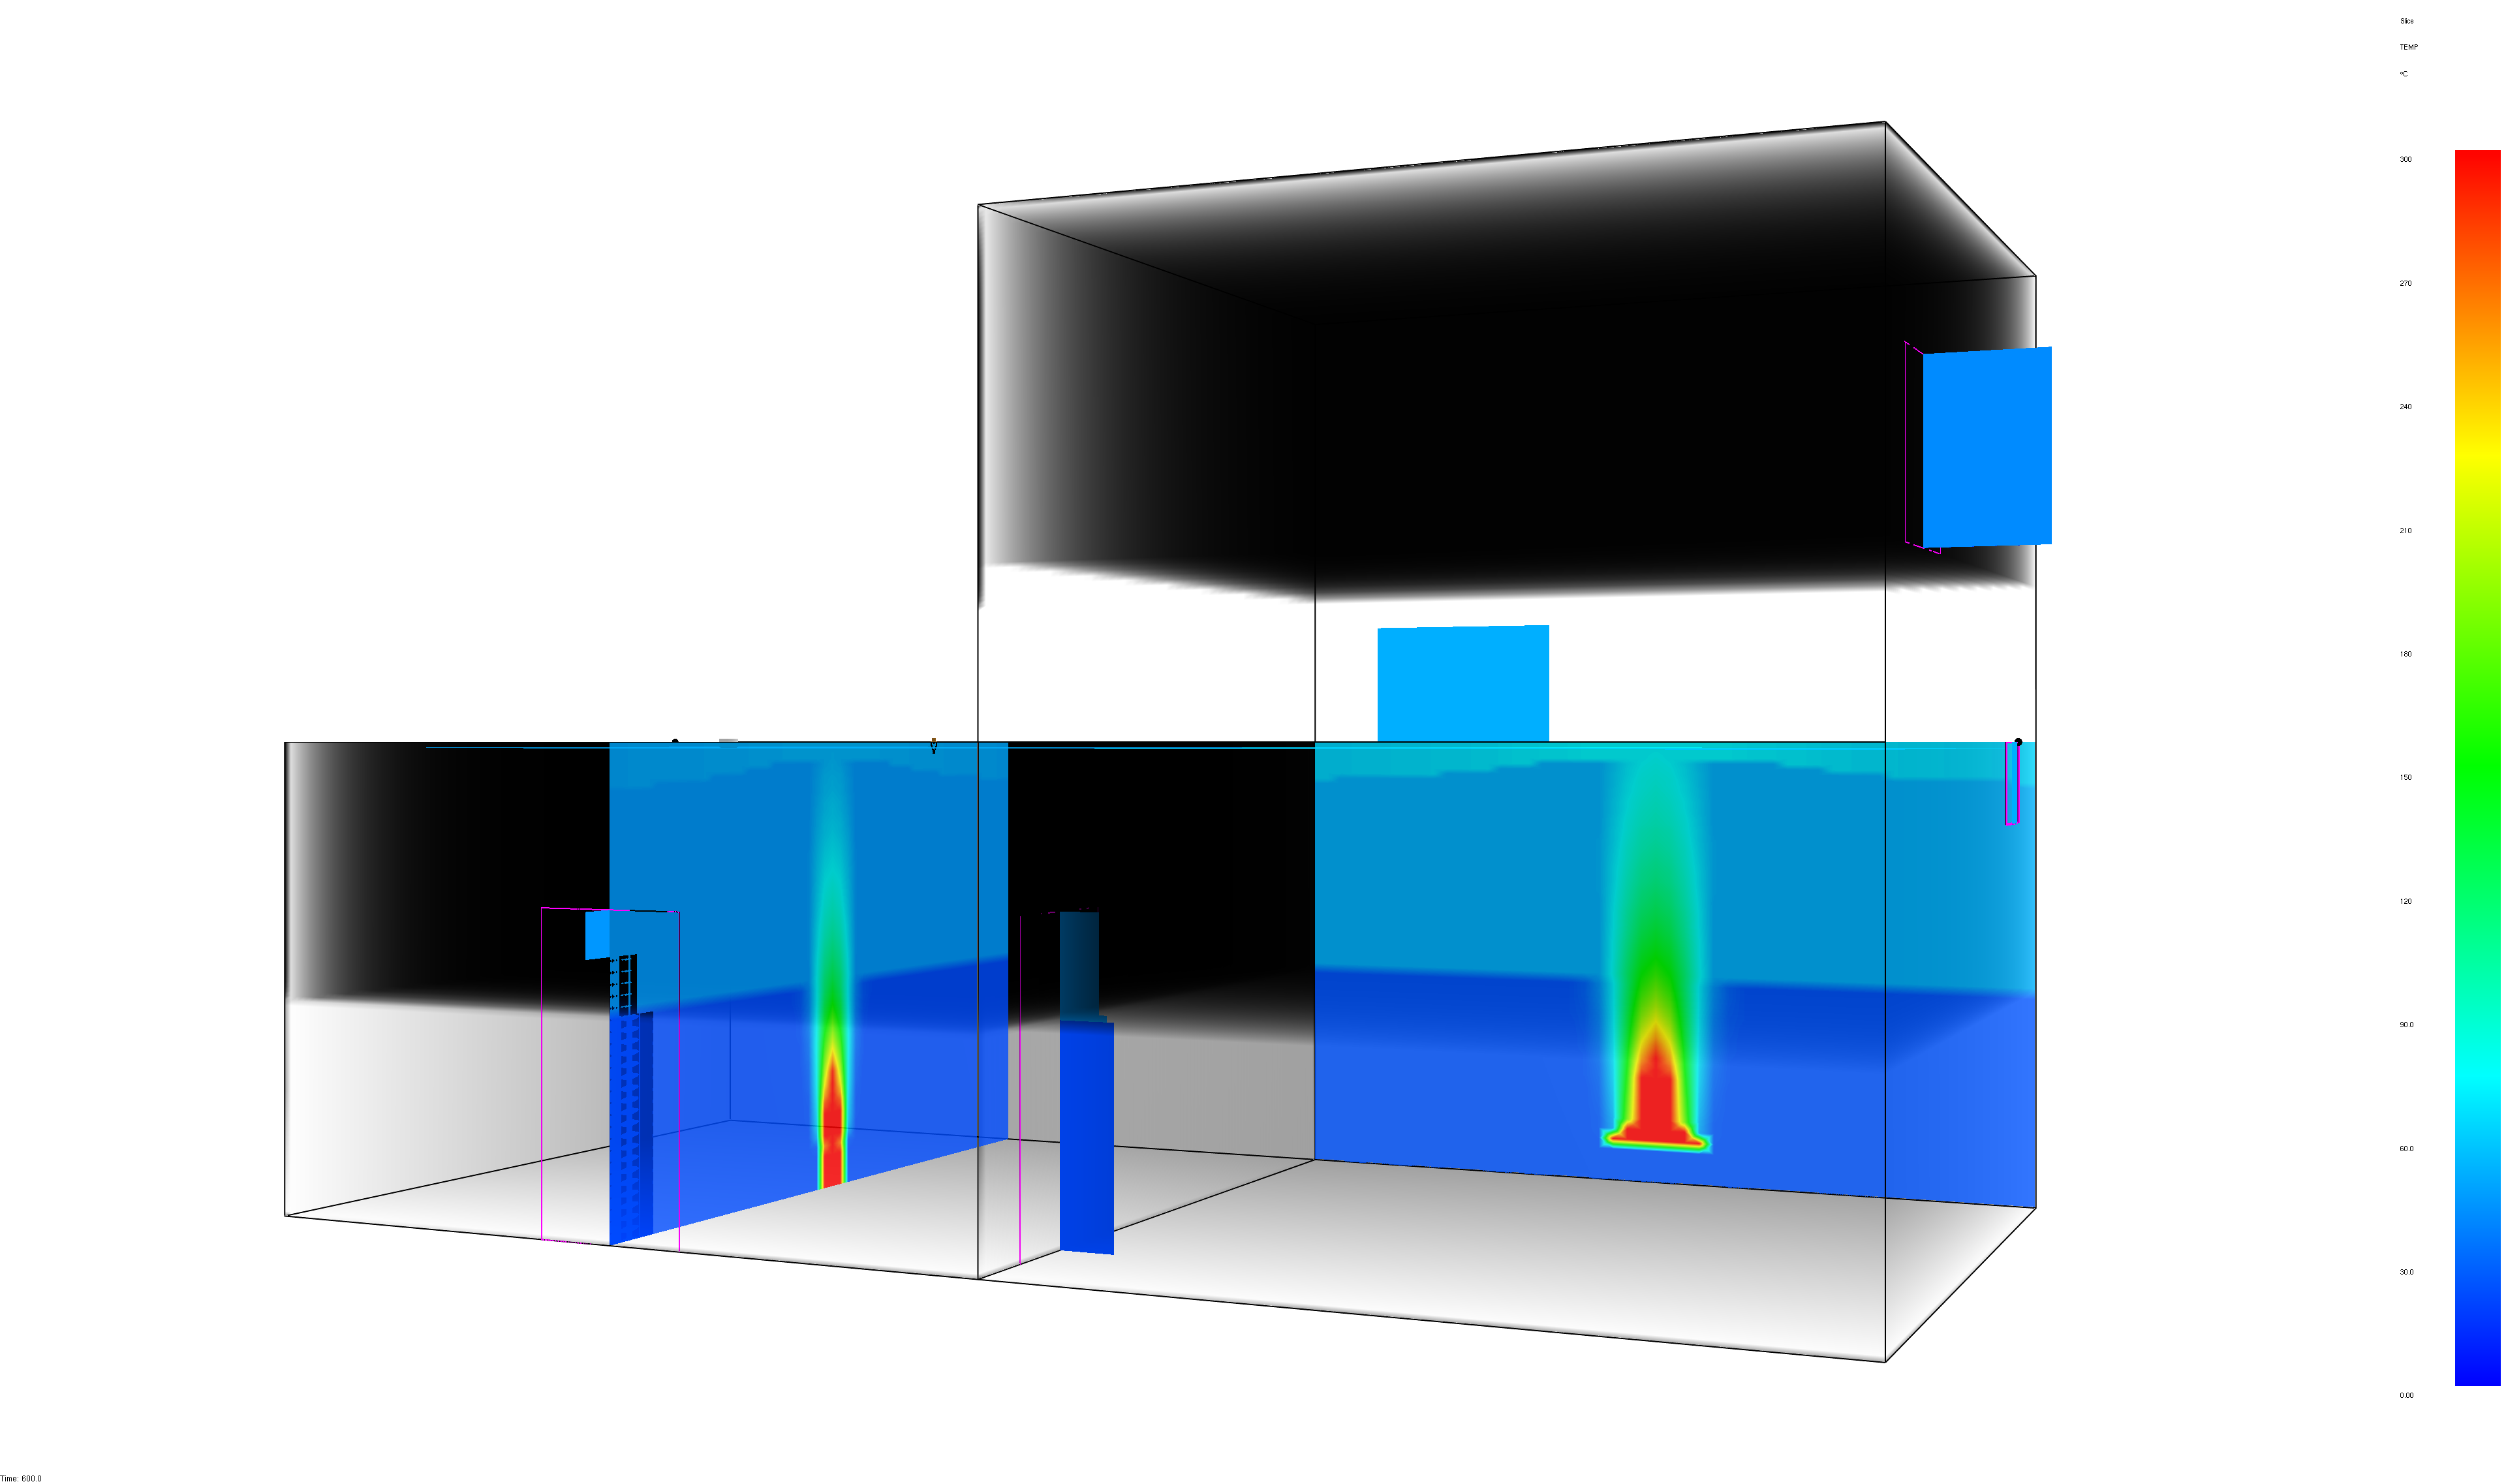
\includegraphics[width=6.5in]{FIGURES/SMV_Sample}
\caption[Example Smokeview Visualization for a Three Compartment Test Case]{Example Smokeview Visualization for a Three Compartment Test Case with Two Fires (\ct{Users_Guide_Example.in})}
\end{center}
\end{figure}

\begin{figure}[h!]
\begin{center}
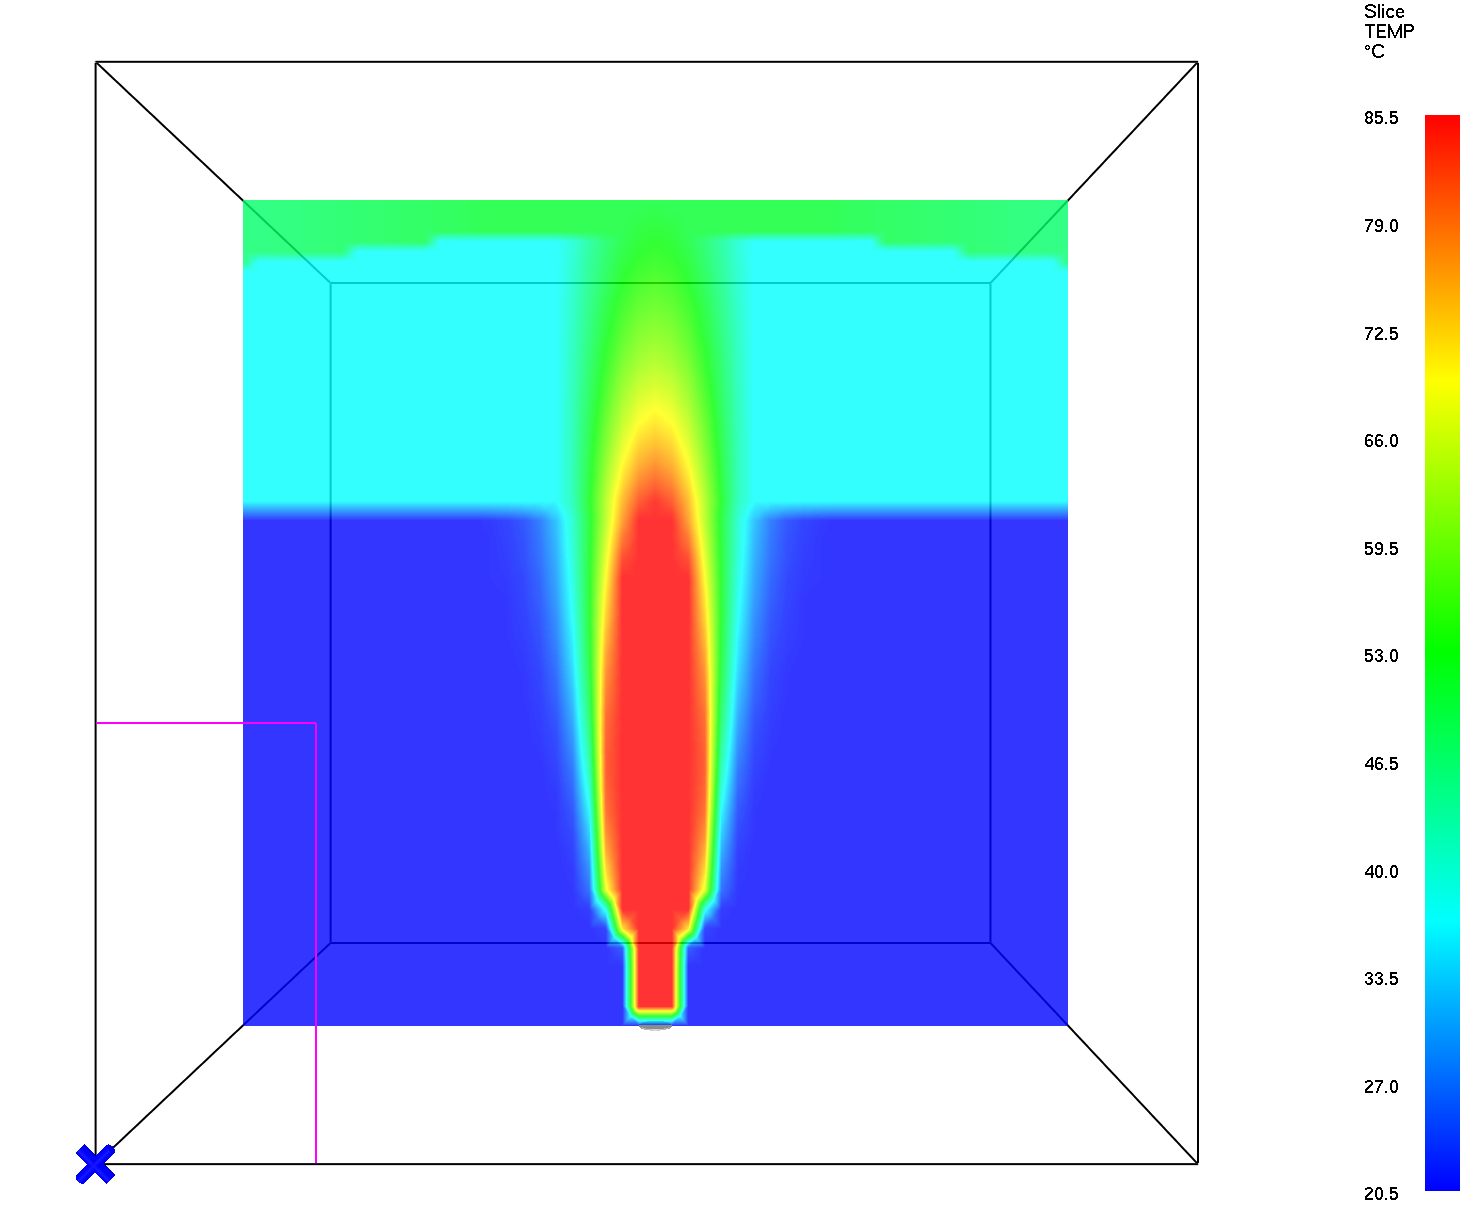
\includegraphics[width=6.5in]{FIGURES/SMV_Temperature}
\caption{Smokeview Visualization of Gas Temperature with a Single Fire}
\end{center}
\end{figure}

\begin{figure}[h!]
\begin{center}
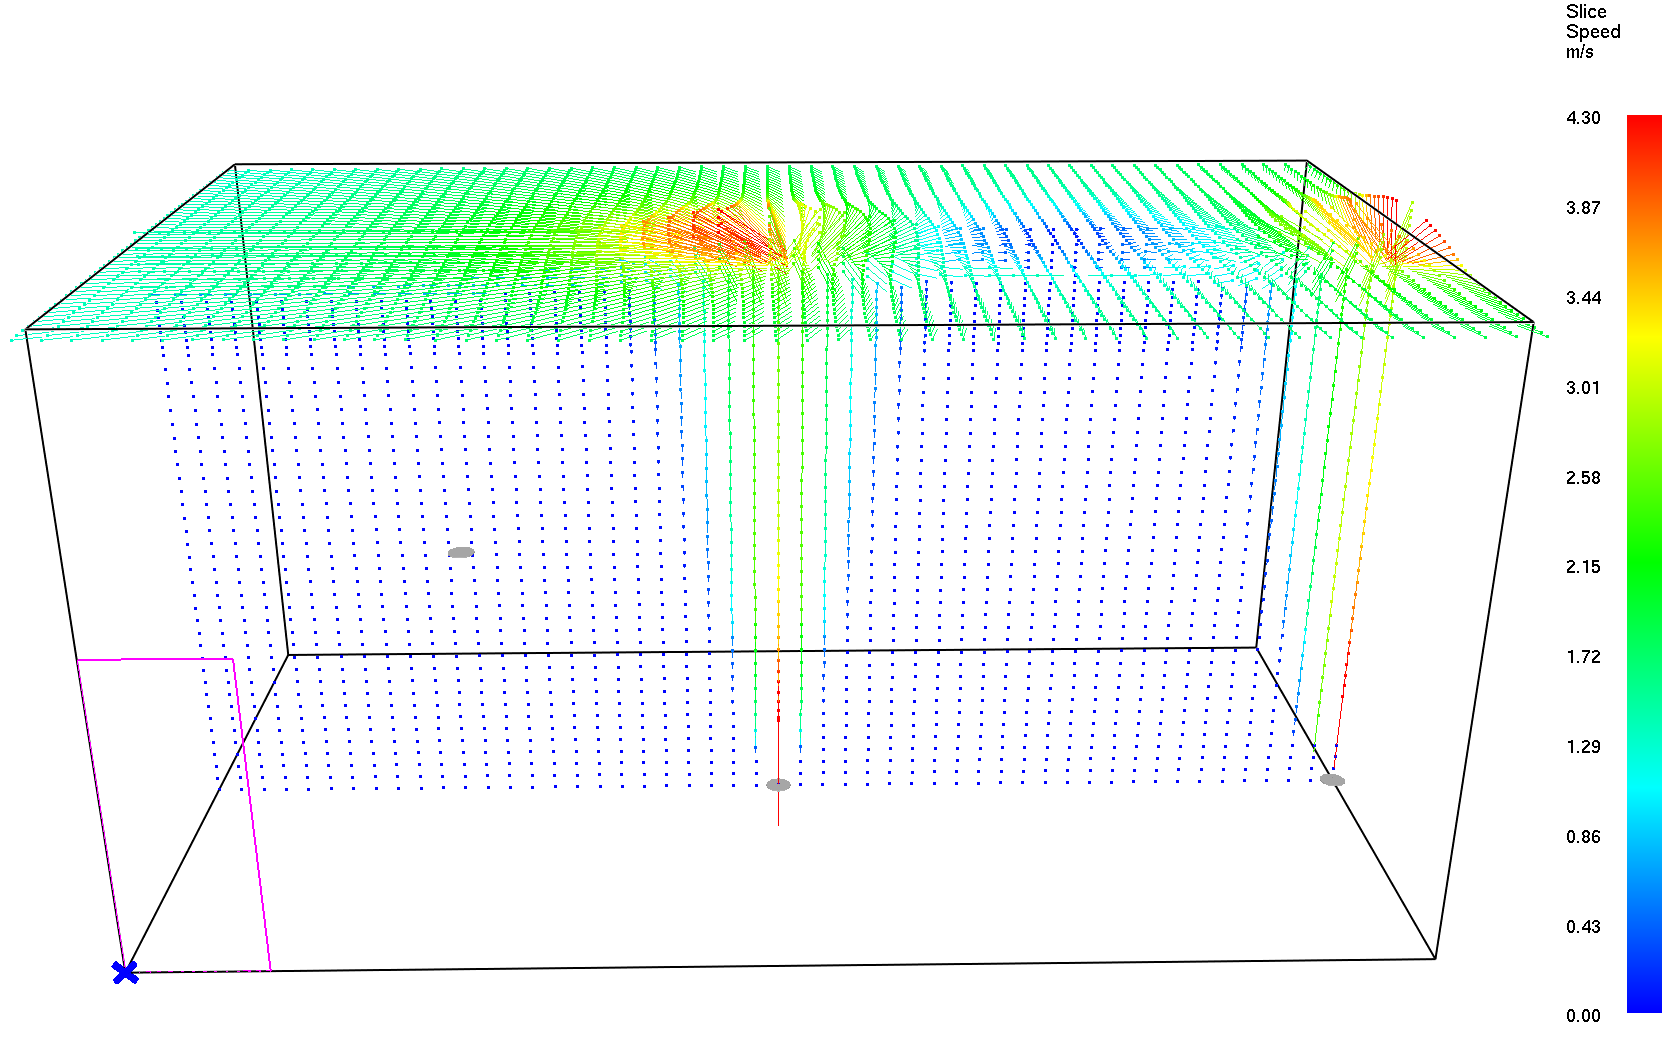
\includegraphics[width=6.5in]{FIGURES/SMV_Velocity}
\caption{Smokeview Visualization of Gas Velocity with Two Fires}
\end{center}
\end{figure}

\begin{figure}[h!]
\begin{center}
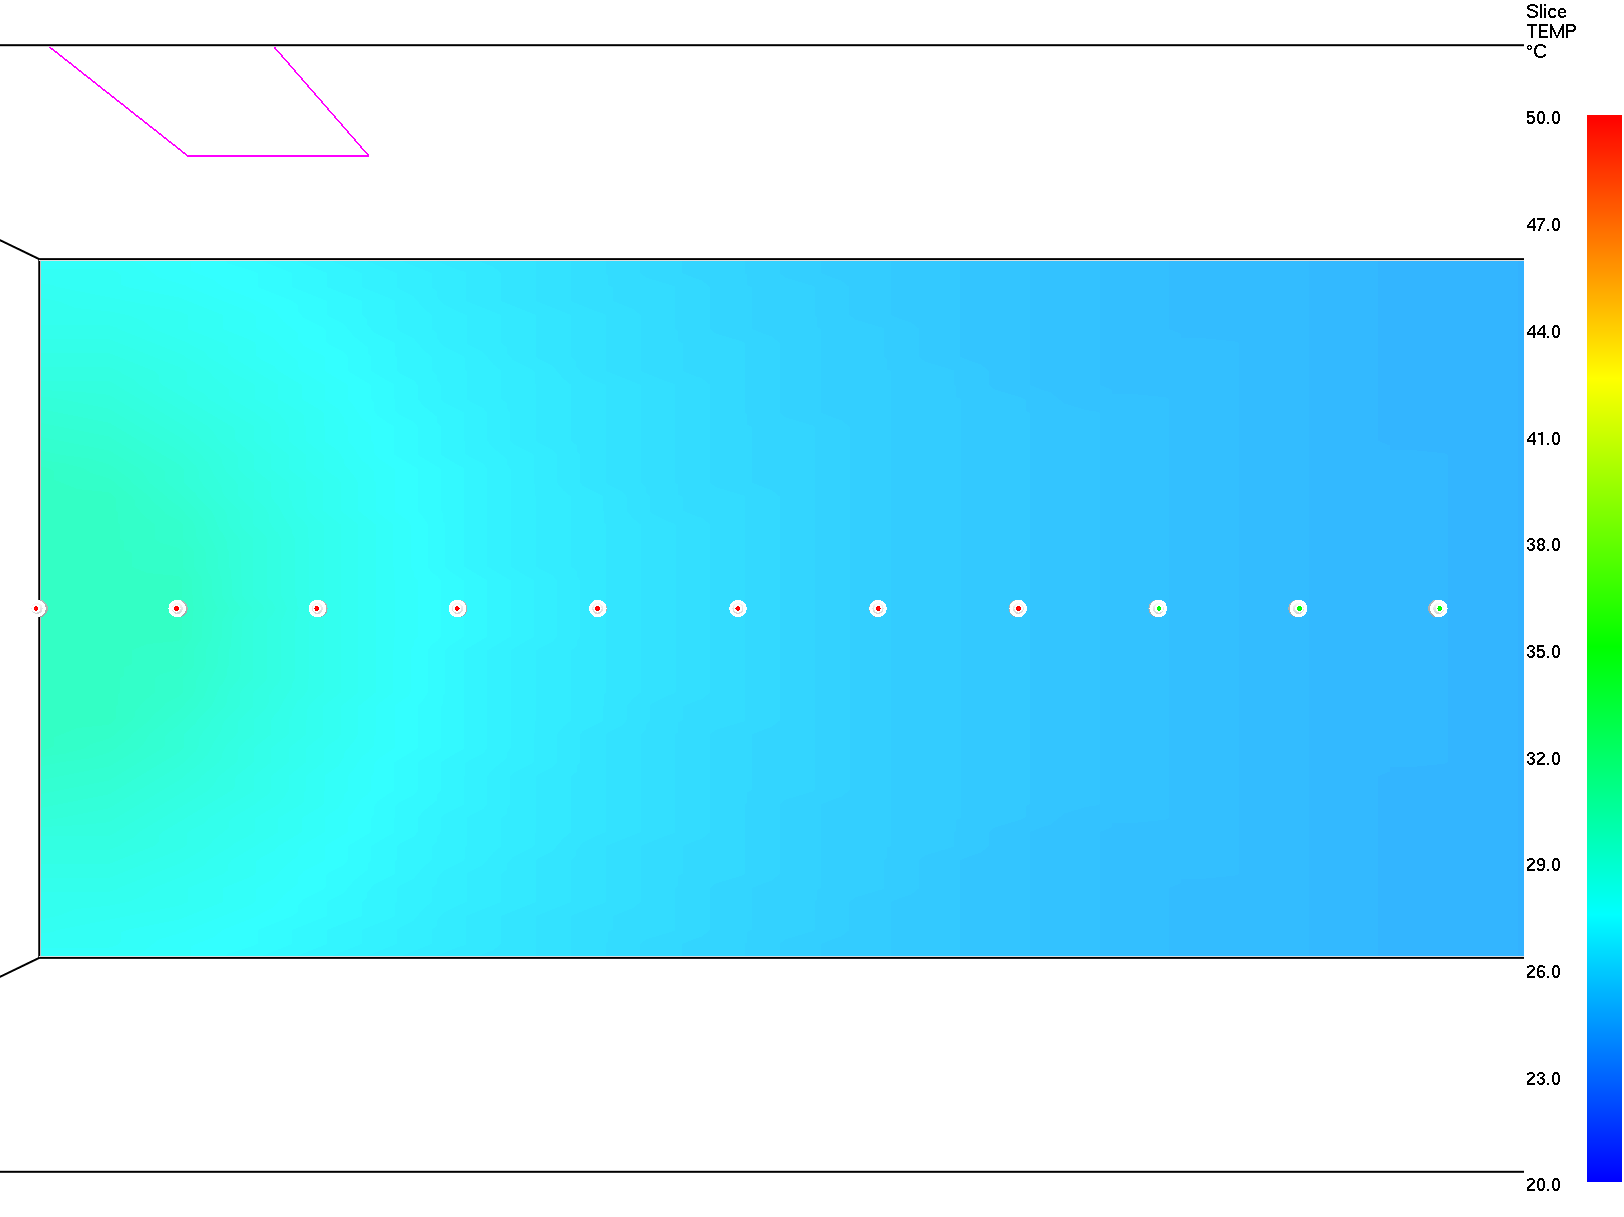
\includegraphics[width=6.5in]{FIGURES/SMV_Detectors}
\caption{Smokeview Visualization of Detector Activation in a Corridor}
\end{center}
\end{figure}

\section{Output Options}

By default, CFAST generates a set of output files that includes a formatted readable output and a set of spreadsheet files.  Options are available to modify the output files.  The default output should be appropriate for most simulations.

\begin{description}
    \item[CFAST Validation Output] If checked, this item directs the CFAST model to output abbreviated headings for spreadsheet columns that are better for automated processing of the data.
    \item[Debug Output] If checked, CFAST will create a detailed output spreadsheet that contains values of all the solution variables at each successful solution time step. This file is typically only of use to model developers diagnosing a problem with the model.
    \item[Show CFAST Window] If checked, this item allows the user to see the Windows command prompt that is used to execute the CFAST model when the Model Simulation, CFAST menu item is used.  By default, this is not checked.  Normally, this can be left unchecked.  For troubleshooting, this can be selected to see additional details of the calculation as it progresses.
\end{description}

\section{Diagnostic Parameters}
\label{info:DIAG}

The \ct{DIAG} namelist is intended for model verification and developer diagnostics, not normal scenarios. Unless noted otherwise, the sub-model switches accept \ct{ON} or \ct{OFF}.
\begin{description}
\item[\texttt{ADIABATIC\_TARGET\_VERIFICATION}] Enables the adiabatic-surface-temperature verification calculation; default \ct{OFF}. When enabled, \ct{RADIATIVE_INCIDENT_FLUX} supplies the imposed flux.
\item[\texttt{CEILING\_JET\_SUB\_MODEL}] Enables the ceiling-jet calculation; default \ct{ON}.
\item[\texttt{CONDUCTION\_SUB\_MODEL}] Enables solid conduction; default \ct{ON}.
\item[\texttt{CONVECTION\_SUB\_MODEL}] Enables convective heat transfer; default \ct{ON}.
\item[\texttt{DASSL\_DEBUG\_PRINT}] Enables DASSL diagnostic output; default \ct{OFF}.
\item[\texttt{DEBUG\_PRINT}] Enables general debug output; default \ct{OFF}.
\item[\texttt{DOOR\_JET\_FIRE\_SUB\_MODEL}] Enables burning in a door jet; default \ct{ON}.
\item[\texttt{ENTRAINMENT\_SUB\_MODEL}] Enables plume entrainment; default \ct{ON}.
\item[\texttt{F}] Gas-temperature values in \unit{\degreeCelsius} for the verification history defined at times \ct{T}; both arrays are required together.
\item[\texttt{FIRE\_SUB\_MODEL}] Enables the fire calculation; default \ct{ON}.
\item[\texttt{GAS\_ABSORBTION\_SUB\_MODEL}] Selects \ct{CALCULATED} gas absorption, the default, or \ct{CONSTANT}. The parameter name retains its source-code spelling.
\item[\texttt{GAS\_TEMPERATURE}] Gas temperature in \unit{\degreeCelsius} for radiation verification. Use with both partial-pressure parameters below.
\item[\texttt{HORIZONTAL\_FLOW\_SUB\_MODEL}] Enables horizontal vent flow; default \ct{ON}.
\item[\texttt{KEYBOARD\_INPUT}] Enables interactive keyboard input during a run; default \ct{ON}.
\item[\texttt{LAYER\_MIXING\_SUB\_MODEL}] Enables interlayer mixing; default \ct{ON}.
\item[\texttt{MECHANICAL\_FLOW\_SUB\_MODEL}] Enables mechanical ventilation flow; default \ct{ON}.
\item[\texttt{MODE}] Reserved compatibility input. The current reader accepts the value but does not use it.
\item[\texttt{OXYGEN\_TRACKING}] Legacy diagnostic switch. In the current reader, \ct{ON} ensures that the fire sub-model remains enabled.
\item[\texttt{PARTIAL\_PRESSURE\_CO2}] CO$_2$ partial pressure in Pa for radiation verification.
\item[\texttt{PARTIAL\_PRESSURE\_H2O}] H$_2$O partial pressure in Pa for radiation verification.
\item[\texttt{RADIATION\_SUB\_MODEL}] Enables thermal radiation; default \ct{ON}.
\item[\texttt{RADIATIVE\_INCIDENT\_FLUX}] Imposed incident flux in \unit{kW/m^2} for adiabatic-target verification; default 0~\unit{kW/m^2}.
\item[\texttt{RAD\_SOLVER}] Set to \ct{RADNNET} to use the neural-network radiation solver; otherwise the standard solver is used.
\item[\texttt{RESIDUAL\_DEBUG\_PRINT}] Enables solver-residual diagnostic output; default \ct{OFF}.
\item[\texttt{STEADY\_STATE\_INITIAL\_CONDITIONS}] Enables steady-state initialization diagnostics; default \ct{OFF}.
\item[\texttt{T}] Times in s corresponding to the verification temperatures in \ct{F}.
\item[\texttt{UPPER\_LAYER\_THICKNESS}] Imposed upper-layer thickness in m for radiation verification.
\item[\texttt{VERIFICATION\_FIRE\_HEAT\_FLUX}] Imposed fire heat flux in \unit{kW/m^2} for verification.
\item[\texttt{VERIFICATION\_TIME\_STEP}] Time step in s used by verification calculations; default 0~S.
\item[\texttt{VERTICAL\_FLOW\_SUB\_MODEL}] Enables vertical vent flow; default \ct{ON}.
\end{description}
